% !Mode:: "TeX:UTF-8"
% !TEX program  = xelatex

%\documentclass{cumcmthesis}
\documentclass[withoutpreface,bwprint]{cumcmthesis} %去掉封面与编号页

\usepackage{url}   % 网页链接
\usepackage{subcaption} % 子标题
\title{全国大学生数学建模竞赛编写的 \LaTeX{} 模板}
\tihao{A}
\baominghao{4321}
\schoolname{XX大学}
\membera{}
\memberb{向左}
\memberc{哈哈}
\supervisor{老师}
\yearinput{2017}
\monthinput{08}
\dayinput{22}

\title{二维Poisson方程的九点差分格式}
\begin{document}
	\maketitle
	~\\
	~\\
	
	作业:
	
	$$
	\left\{
	\begin{array}{lcl}
	-(\dfrac{\partial^{2}{u}}{\partial{x^{2}}}+\dfrac{\partial^{2}{u}}{\partial{y^{2}}})=(\pi^{2}-1)e^{x}sin(\pi y) &,&0 \leq x \leq 2,0 \leq y \leq 1 \\
	
	u(0,y)=sin(\pi y),u(2,y)=e^{2}sin(\pi y) &, & 0 \leq y \leq 1 \\
	
	u(x,0)=0,u(x,1)=0,&, &0 \leq x \leq 2
	\end{array}
	\right.
	$$
	
	该问题的精确解为$ u(x,y)=e^{x}sin(\pi y)$.
	
	定义误差为$$ E(h_{1},h_{2})=\max \limits_{1 \leq i \leq M-1 \atop 1 \leq j \leq N-1 } |u(x_{i},y_{j})-u_{ij})| $$
	
	请分析误差在不同步长下的变化情况,验证误差阶,并画出误差图。

	
	
	解:将xM等分,将yN等分。
	
	九点差分格式为
	\begin{equation*}
	\begin{split}
	&-k_{1}u_{i-1,j-1}+(2k_{1}-k_{2})u_{i-1,j}-k_{1}u_{i-1,j+1}+(2k_{1}-k_{3})u_{i,j-1}+(2k_{2}+2k_{3}-4k_{1})u_{i,j} +\\
	&(2k_{1}-k_{3})u_{i,j+1}-k_{1}u_{i+1,j-1}+(2k_{1}-k_{2})u_{i+1,j}-k_{1}u_{i+1,j+1}\\
	&=f_{i,j}+\dfrac{1}{12}[h_{1}^{2}\dfrac{\partial^{2}{f}}{\partial{x}^{2}}(x_{i},y_{j})+h_{2}^{2}\dfrac{\partial^{2}{f}}{\partial{y}^{2}}(x_{i},y_{j})]
	\end{split}
	\end{equation*}
	
	其中,$ 1 \leq i \leq N-1 ,1 \leq j \leq N-1 $.
	$f=(\pi^{2}-1)e^{x}sin(\pi y)$.
	
	$k_{1}=\dfrac{h_{1}^{2}+h_{2}^{2}}{12h_{1}^{2}h_{2}^{2}}$,$k2=\dfrac{1}{h_{1}^{2}}$,$ k3=\dfrac{1}{h_{2}^{2}} $
    ~\\
    
	可用高斯-塞德尔迭代解方程组,迭代式写为
	\begin{equation*}
	\begin{split}
		&u_{i,j}^{k+1}=\{f_{i,j}+\dfrac{1}{12}[h_{1}^{2}\dfrac{\partial^{2}{f}}{\partial{x}^{2}}(x_{i},y_{j})+h_{2}^{2}\dfrac{\partial^{2}{f}}{\partial{y}^{2}}(x_{i},y_{j})]+\\
		&k_{1}u_{i-1,j-1}^{k+1}-(2k_{1}-k_{2})u_{i-1,j}^{k+1}+k_{1}u_{i-1,j+1}^{k+1}-(2k_{1}-k_{3})u_{i,j-1}^{k+1}-\\
		&(2k_{1}-k_{3})u_{i,j+1}^{k}+k_{1}u_{i+1,j-1}^{k}-(2k_{1}-k_{2})u_{i+1,j}^{k}+k_{1}u_{i+1,j+1}^{k} \}/ (2k_{2}+2k_{3}-4k_{1})
	\end{split}
	\end{equation*}

	
	$k$表示第k次迭代
	
	~\\
	~\\
	
	
	\textbf{解题程序运行于Matlab 2018a.}
	
	当$h_{1}=\dfrac{1}{20}$,$h_{2}=\dfrac{1}{20}$时的数值解和精确解对比见图\ref{fig:f5},从图像上看很接近。
	\begin{figure}
		\centering
		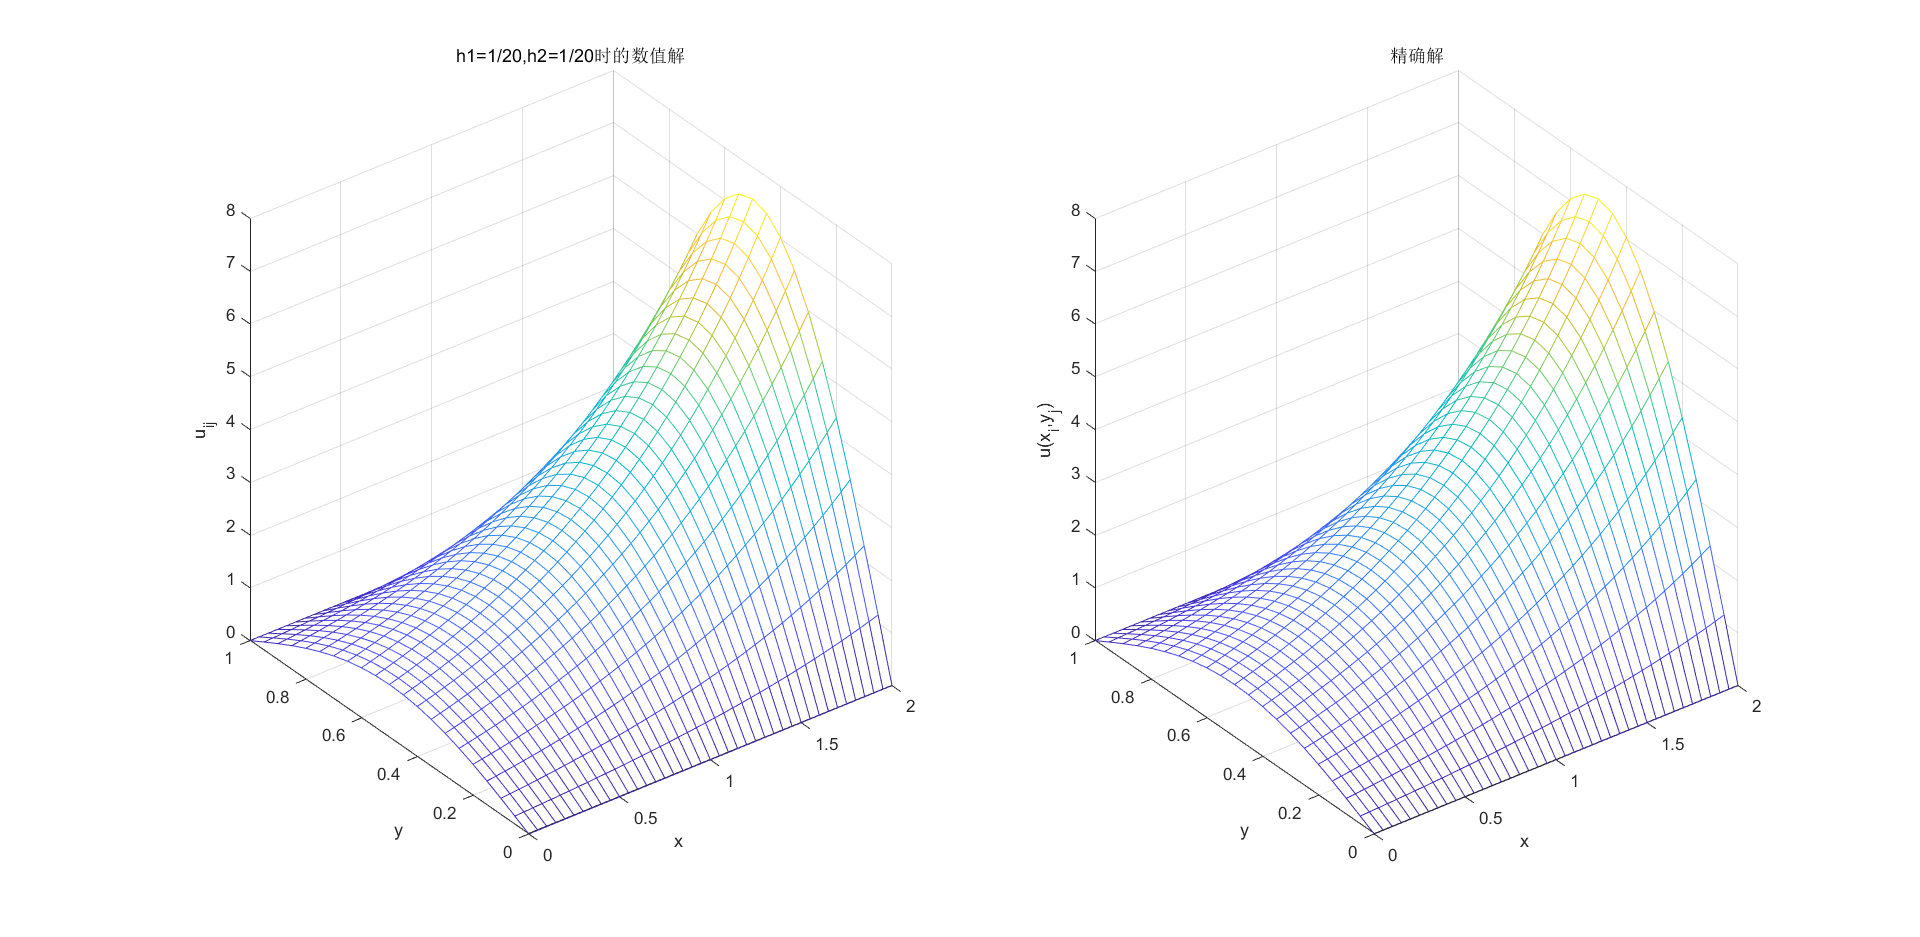
\includegraphics[width=1\linewidth]{figures/f5}
		\caption{$h_{1}=\dfrac{1}{20}$,$h_{2}=\dfrac{1}{20}$时的数值解和精确解}
		\label{fig:f5}
	\end{figure}
	
	当取不同的$h_{1}$和$h_{2}$时,数值解在一些点上的取值和精确解见表\ref{tab:1},可知,步长越小,数值解越逼近于精确解。
	% Table generated by Excel2LaTeX from sheet 'Sheet1'
	\begin{table}[htbp]
		\centering
		\caption{不同步长下的数值解和精确解}
		\begin{tabular}{crrrr}
			\toprule[1.5pt]
			\multirow{2}[0]{*}{$h_{1}$,$h_{2}$} & \multicolumn{4}{c}{x(y=0.5时)} \\
			& \multicolumn{1}{c}{0.4} & \multicolumn{1}{c}{0.8} & \multicolumn{1}{c}{1.2} & \multicolumn{1}{c}{1.6} \\
			\midrule[1pt]
			1/10,1/10 & 1.4918055414  & 2.2255083825  & 3.3200724539  & 4.9529855650  \\
			1/20,1/20 & 1.4918235062  & 2.2255389042  & 3.3201141569  & 4.9530295099  \\
			1/40,1/40 & 1.4918246233  & 2.2255408021  & 3.3201167501  & 4.9530322425  \\
			1/80,1/80 & 1.4918246930  & 2.2255409206  & 3.3201169119  & 4.9530324130  \\
			精确解   & 1.4918246976  & 2.2255409285  & 3.3201169227  & 4.9530324244  \\
			\bottomrule[1.5pt]
		\end{tabular}%
		\label{tab:1}%
	\end{table}%

	
	
	取不同$h_{1}$和$h_{2}$时,误差见图\ref{fig:2},$h_{1}$和$h_{2}$越小,误差越小。
	
	 \begin{figure*}
		\centering
		\begin{subfigure}[b]{0.48\textwidth}
			\centering
			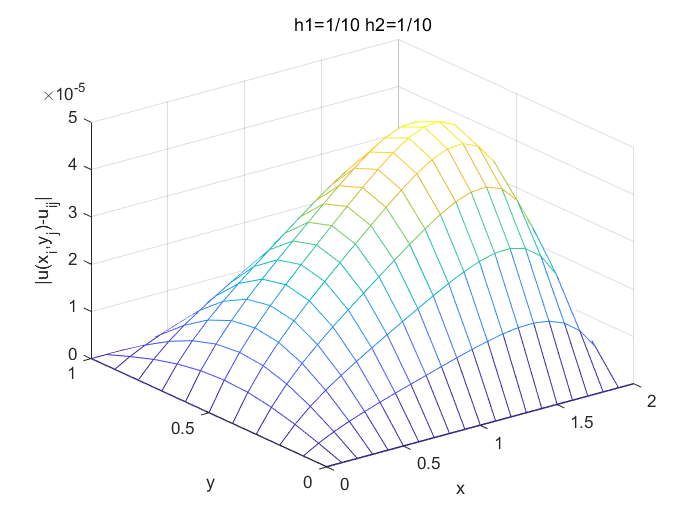
\includegraphics[width=\textwidth]{figures/f1}
			\caption[Network2]%
			{{\small $h_{1}=1/10$,$h_{2}=1/10$时的误差}}    
			\label{fig:mean and std of net14}
		\end{subfigure}
		\hfill
		\begin{subfigure}[b]{0.48\textwidth}  
			\centering 
			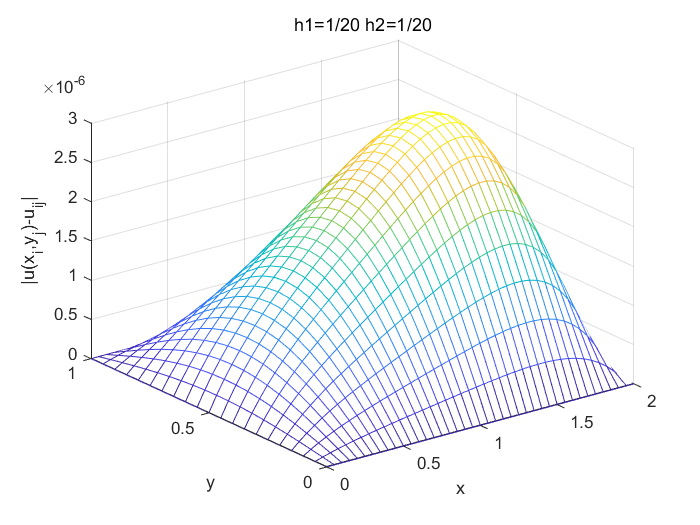
\includegraphics[width=\textwidth]{figures/f2}
			\caption[]%
			{{\small $h_{1}=1/20$,$h_{2}=1/20$时的误差}}    
			\label{fig:mean and std of net24}
		\end{subfigure}
		\vskip\baselineskip
		\begin{subfigure}[b]{0.48\textwidth}   
			\centering 
			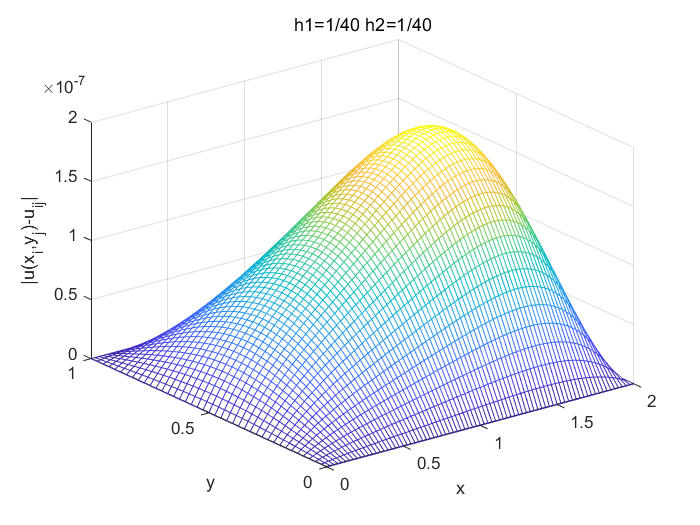
\includegraphics[width=\textwidth]{figures/f3}
			\caption[]%
			{{\small $h_{1}=1/40$,$h_{2}=1/40$时的误差}}    
			\label{fig:mean and std of net34}
		\end{subfigure}
		\quad
		\begin{subfigure}[b]{0.48\textwidth}   
			\centering 
			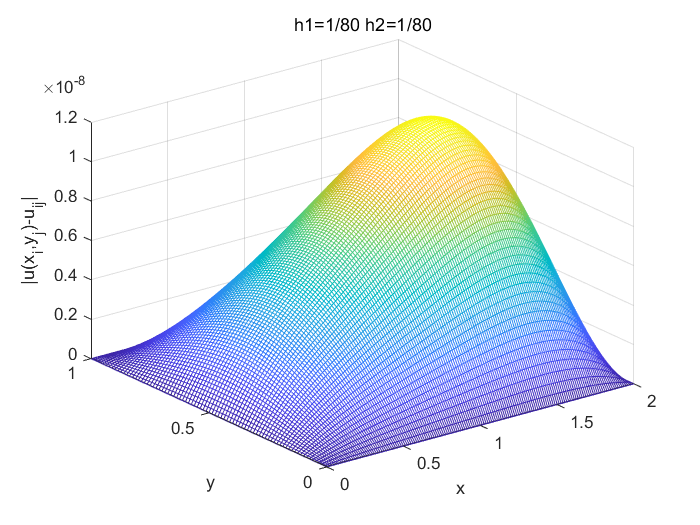
\includegraphics[width=\textwidth]{figures/f4}
			\caption[]%
			{{\small $h_{1}=1/80$,$h_{2}=1/80$时的误差}}    
			\label{fig:mean and std of net44}
		\end{subfigure}
		\caption[ The average and standard deviation of critical parameters ]
		{ 取不同$h_{1}$,$h_{2}$时的误差} 
		\label{fig:2}
	\end{figure*}


	定义误差阶为
	$$rate=log_{2}(E(2h_{1},2h_{2})/E(h_{1},h_{2}))$$
	
	
	$h_{1} =h_{2}$时的误差阶见表\ref{tab:2},$h_{1} < h_{2}$时的误差阶见表\ref{tab:3},$h_{1} >h_{2}$时的误差阶见表\ref{tab:4},误差均达到了4阶,而五点差分格式的精度只有2阶,因此,九点差分的精度高于五点差分格式。
	% Table generated by Excel2LaTeX from sheet 'Sheet1'
	\begin{table}[htbp]
		\centering
		\caption{$h_{1}=h_{2}$时最大误差和误差阶}
		\begin{tabular}{crr}
			\toprule[1.5pt]
			\multirow{2}[0]{*}{$h_{1},h_{2}$} & \multicolumn{1}{c}{\multirow{2}[0]{*}{$E(h_{1},h_{2})$}} & \multicolumn{1}{c}{\multirow{2}[0]{*}{rate}} \\
			&       &  \\
			\midrule[1pt]
			$\frac{1}{10},\frac{1}{10}$ & 4.84E-05 & \multicolumn{1}{c}{*} \\
			$\frac{1}{20},\frac{1}{20}$ & 3.01E-06 & 4.005469 \\
			$\frac{1}{40},\frac{1}{40}$ & 1.88E-07 & 4.000988 \\
			$\frac{1}{80},\frac{1}{80}$ & 1.18E-08 & 3.999005 \\
			\bottomrule[1.5pt]
		\end{tabular}%
		\label{tab:2}%
	\end{table}%

	% Table generated by Excel2LaTeX from sheet 'Sheet1'
	\begin{table}[htbp]
		\centering
		\caption{$h_{1}<h_{2}$时最大误差和误差阶}
		\begin{tabular}{lrc}
			\toprule[1.5pt]
			\multicolumn{1}{c}{\multirow{2}[0]{*}{$h_{1},h_{2}$}} & \multicolumn{1}{c}{\multirow{2}[0]{*}{$E(h_{1},h_{2})$}} & \multirow{2}[0]{*}{rate} \\
			&       &  \\
			\midrule[1pt]
			$\frac{1}{20},\frac{1}{5}$ & 1.01E-03 & * \\
			$\frac{1}{40},\frac{1}{10}$ & 6.53E-05 & 3.956884  \\
			$\frac{1}{80},\frac{1}{20}$ & 4.06E-06 & 4.007516  \\
			$\frac{1}{160},\frac{1}{40}$ & 2.54E-07 & 4.001663  \\
			\bottomrule[1.5pt]
		\end{tabular}%
		\label{tab:3}%
	\end{table}%
	
	% Table generated by Excel2LaTeX from sheet 'Sheet1'
	\begin{table}[htbp]
		\centering
		\caption{$h_{1}>h_{2}$时最大误差和误差阶}
		\begin{tabular}{lrc}
			\toprule[1.5pt]
			\multicolumn{1}{c}{\multirow{2}[0]{*}{$h_{1},h_{2}$}} & \multicolumn{1}{c}{\multirow{2}[0]{*}{$E(h_{1},h_{2})$}} & \multirow{2}[0]{*}{rate} \\
			&       &  \\
			\midrule[1pt]
			$\frac{1}{5},\frac{1}{20}$ & 1.87E-05 & * \\
			$\frac{1}{10},\frac{1}{40}$ & 1.18E-06 & 3.990484  \\
			$\frac{1}{20},\frac{1}{80}$ & 7.37E-08 & 3.997730  \\
			$\frac{1}{40},\frac{1}{160}$ & 4.63E-09 & 3.991979  \\
			\bottomrule[1.5pt]
		\end{tabular}%
		\label{tab:4}%
	\end{table}%
	
	
\end{document}